\begin{figure*}[h]
  \centering
  \begin{minipage}{.5\textwidth}
    \centering
    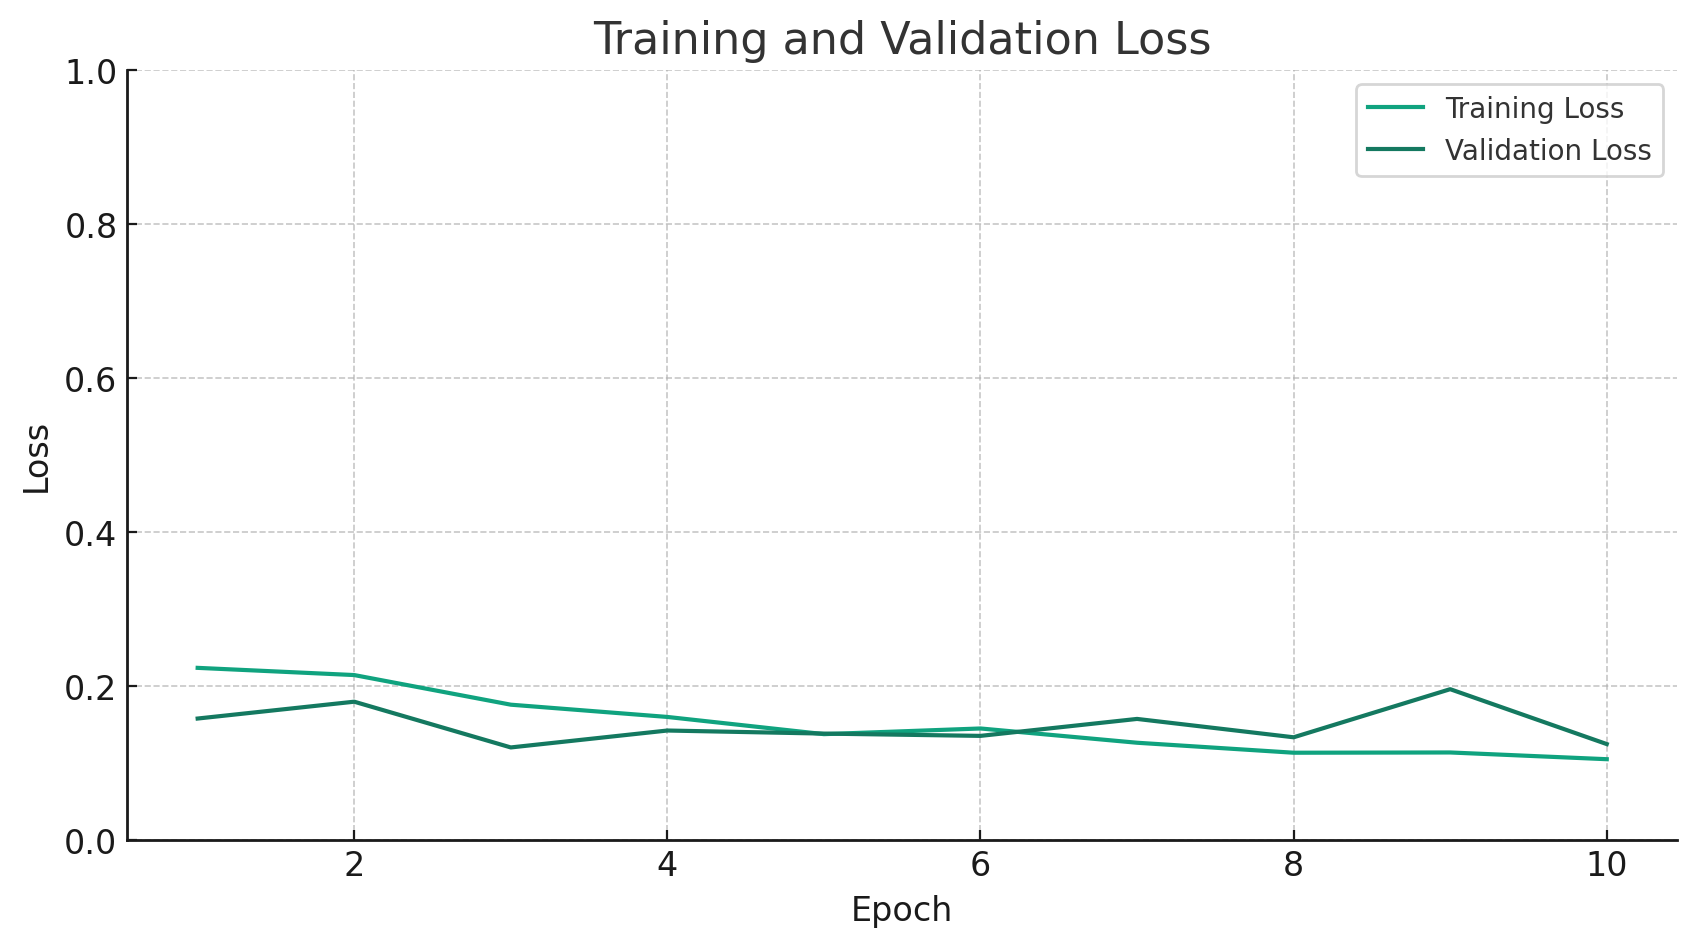
\includegraphics[scale=0.4]{Images/Loss.jpg}
    \caption{Loss per Epoch}
    \label{fig:loss}
  \end{minipage}%
  \begin{minipage}{.5\textwidth}
    \centering
    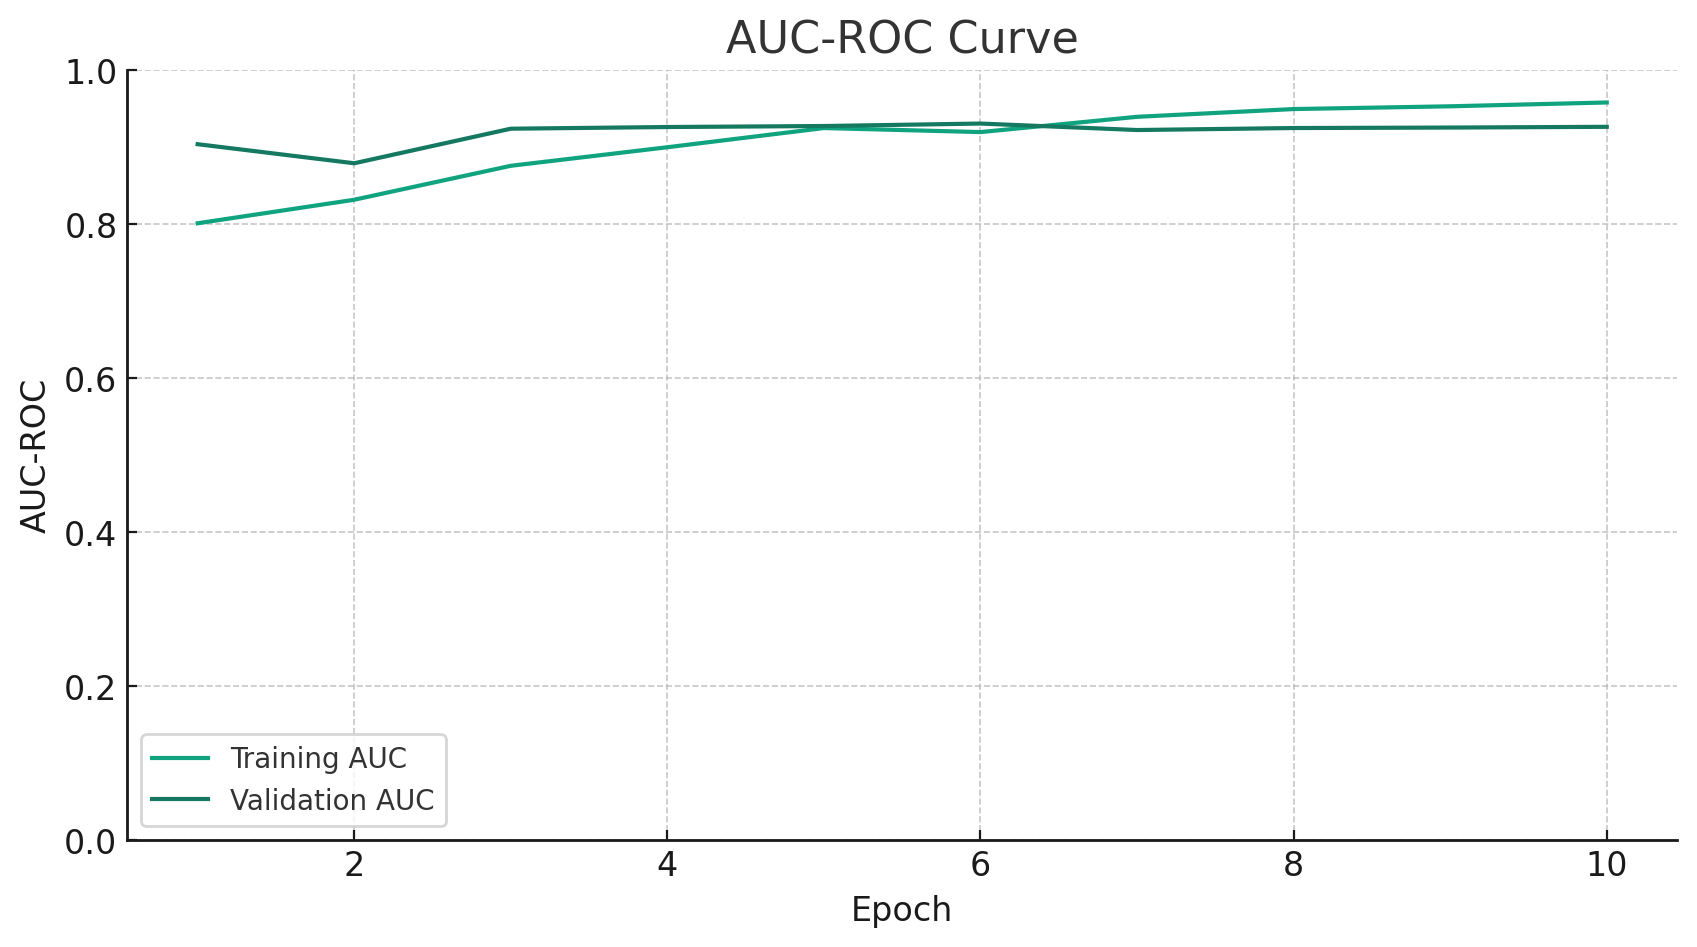
\includegraphics[scale=0.4]{Images/AUC-ROC.jpg}
    \caption{AUC-ROC Score per Epoch}
    \label{fig:auc-roc}
  \end{minipage}
\end{figure*}

The goal of this project was to accurately classify the severity of diabetic retinopathy in fundus camera images and to generate a saliency map highlighting the image regions influencing the classification decision. We evaluated model performance using cross-entropy loss and the Area Under the Receiver Operating Characteristic Curve (AUC-ROC). Due to significant class imbalance, we chose AUC-ROC over accuracy as a performance metric. Since AUC-ROC remains unaffected by skewed class distributions, it provides a more reliable indicator of model efficacy than accuracy. Additionally, the AUC-ROC curve is influenced by the balance between sensitivity and specificity, ensuring that the abundance of Class 0 cases does not skew the performance metric.

\autoref{fig:loss} illustrates the training and validation loss trends. Notably, at around 10 epochs, both training and validation losses converge to approximately 0.15. While the training loss continues to decrease, the validation loss begins to fluctuate after a few epochs. To prevent overfitting and manage computational resources efficiently, we limited our training to 10 epochs.

\autoref{fig:auc-roc} displays the AUC-ROC for both training and validation sets, which begin to plateau at about the fifth epoch, peaking near 0.9. This indicates a 90\% probability that the model accurately distinguishes between the two classes, confirming the model's robust performance in assessing the severity of diabetic retinopathy and achieving our primary objective.

Our secondary objective involves visually identifying the critical areas influencing the model's decisions. \autoref{fig:dr0} presents a saliency map for an image classified as Class 0 (No Diabetic Retinopathy), where the focus is primarily on three regions. The top left and bottom left corners are examined for notches indicating mirrored images. The right-hand focus assesses the blood vessels for abnormal vascularization and hemorrhaging. Conversely, \autoref{fig:dr4} shows a saliency map for Class 4 (Proliferative Diabetic Retinopathy), with particular attention to neovascularization driven by angiogenesis and hemorrhaging. Notably, the model disregards a large dark spot in the upper left quadrant, which we identified as a choroidal nevus — a benign, commonly occurring pigmented lesion unrelated to diabetic retinopathy \cite{noauthor_distinguishing_2012}. This discernment demonstrates the model's capability to distinguish between relevant and unrelated features, which we consider satisfactory for our second objective. However, a comprehensive assessment of the model's performance across various features would require extensive clinical annotation.

\begin{figure*}[t]
  \centering
  \begin{minipage}{\textwidth}
    \centering
    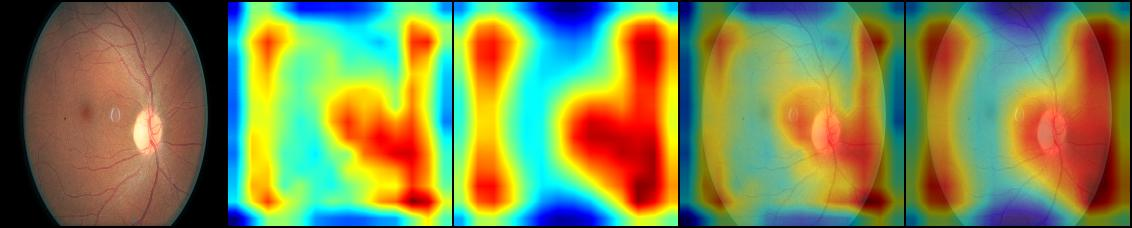
\includegraphics[scale=0.4]{Images/20_left.jpeg}
    \caption{Saliency Map for an Image with No Diabetic Retinopathy}
    \label{fig:dr0}
  \end{minipage}%
\end{figure*}

\begin{figure*}[t]
  \centering
  \begin{minipage}{\textwidth}
    \centering
    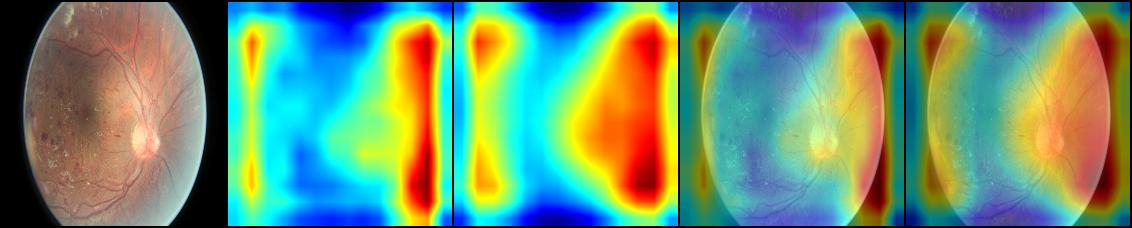
\includegraphics[scale=0.4]{Images/16_left.jpeg}
    \caption{Saliency Map for an Image with Proliferative Diabetic Retinopathy}
    \label{fig:dr4}
  \end{minipage}%
\end{figure*}